% (The MIT License)
%
% Copyright (c) 2022-2023 Yegor Bugayenko
%
% Permission is hereby granted, free of charge, to any person obtaining a copy
% of this software and associated documentation files (the 'Software'), to deal
% in the Software without restriction, including without limitation the rights
% to use, copy, modify, merge, publish, distribute, sublicense, and/or sell
% copies of the Software, and to permit persons to whom the Software is
% furnished to do so, subject to the following conditions:
%
% The above copyright notice and this permission notice shall be included in all
% copies or substantial portions of the Software.
%
% THE SOFTWARE IS PROVIDED 'AS IS', WITHOUT WARRANTY OF ANY KIND, EXPRESS OR
% IMPLIED, INCLUDING BUT NOT LIMITED TO THE WARRANTIES OF MERCHANTABILITY,
% FITNESS FOR A PARTICULAR PURPOSE AND NONINFRINGEMENT. IN NO EVENT SHALL THE
% AUTHORS OR COPYRIGHT HOLDERS BE LIABLE FOR ANY CLAIM, DAMAGES OR OTHER
% LIABILITY, WHETHER IN AN ACTION OF CONTRACT, TORT OR OTHERWISE, ARISING FROM,
% OUT OF OR IN CONNECTION WITH THE SOFTWARE OR THE USE OR OTHER DEALINGS IN THE
% SOFTWARE.

\documentclass{article}
\usepackage[T2A,T1]{fontenc}
\usepackage[utf8]{inputenc}
\usepackage{CJKutf8} % for chinese font
\usepackage{../ppa}
\newcommand*\thetitle{Program Analysis}
\newcommand*\thesubtitle{Metrics, Soundness, Lattices, AI}
\begin{document}

\plush{\lnTitlePage{6}{10}{ItJwyiUFjrs}}

\pptToc

\plush{\pptChapter{Basics}}

\pptSection[Property]{Syntactic \& Semantic Properties}

\emph{Semantic} property can be completely defined with respect to the set of executions of a program,
while a \emph{syntactic} property can be decided directly based on the program text.

{\ttfamily if (x) \{ printf(\begin{CJK}{UTF8}{gbsn}"大家好"\end{CJK}); \}}

Which properties are dynamic?
\begin{itemize}\setlength\itemsep{0pt}
\item A program may print a text to the console
\item A program may call \texttt{printf()} C library function
\item A program prints to the console
\item A program consists of one line of code
\end{itemize}

\plush{}

\pptSection[Rice]{Rice's Theorem}

\emph{Rice's theorem} states that all non-trivial semantic properties of programs are undecidable.

A property is \emph{non-trivial} if it is neither true for every partial computable function, nor false for every partial computable function.

\emph{Halting problem} is the problem of determining, from 1)~a description of an arbitrary computer program and 2)~an input, whether the program will finish running, or continue to run forever. A general algorithm to solve the halting problem for all possible program–input pairs \textbf{cannot exist}.

\plush{}

\pptSection[Non-trivial]{Non-trivial Properties}

Examples of a non-trivial properties:

\begin{itemize}\setlength\itemsep{0pt}
\item A program exits
\item A program prints ``Hello''
\item A program finishes in less than 5 seconds
\item A program dies with ``Segmentation Fault''
\item A program prints user password to the console
\end{itemize}

Suggest a few properties.

\plush{}

\pptSection[Static]{Static Analysis}

Consider two C++ programs given to a \emph{static analyzer} (e.g. \href{https://clang.llvm.org/extra/clang-tidy/}{Clang Tidy}):

\begin{multicols}{2}
{\ttfamily
int f() \{ \\
\quad int x = 0; \\
\quad return 42 / x; \\
\}}
\par\columnbreak\par
{\ttfamily
int f(int x) \{ \\
\quad return 42 / x; \\
\}}
\end{multicols}

Expected answers from Clang Tidy:

\begin{multicols}{2}
\textcolor{green}{\textbf{Yes! :)}}
\par\columnbreak\par
\textcolor{red}{\textbf{No :(}}
\end{multicols}

\plush{}

\pptSection[Style]{Style Checking}

Consider two C++ programs given to a \emph{style checker} (e.g. \href{https://github.com/cpplint/cpplint}{cpplint}):

\begin{multicols}{2}
{\ttfamily
int f (int x) \\
\{ \\
\quad return 42 / x; \\
\}}
\par\columnbreak\par
{\ttfamily
int foo(int x) \{ \\
\quad return 42 / x; \\
\}}
\end{multicols}

Expected answers from cpplint:

\begin{multicols}{2}
\textcolor{green}{{\ttfamily Extra space before ( in function call ; \{ should almost always be at the end of the previous line}}
\par\columnbreak\par
\textcolor{red}{\textbf{No :(}}
\end{multicols}

\plush{}

\pptSection[Dynamic]{Dynamic Analysis}

Consider this C++ program (Clang Tidy finds no issues) given to a \emph{dynamic analyzer}
(\href{https://en.wikipedia.org/wiki/Code_sanitizer}{AddressSanitizer}):

\begin{pptWideOne}
\begin{multicols}{2}
{\ttfamily
int foo(int i) \{ \\
\quad int a[5]; \\
\quad return a[i]; \\
\} \\
int main() \{ \\
\quad return foo(6); \\
\}}
\par\columnbreak\par
{\ttfamily
\$ gcc -fsanitize=address -g a.cpp \\
\$ ./a.out}

\pptPic{1}{address.png}
\end{multicols}
\end{pptWideOne}

Dynamic analysis == testing.

\plush{}

\plush{\pptChapter[Quality]{Quality of Analysis}}

\pptSection[Sound]{Sound \& Complete}

\pptPic{0.8}{sound-complete.jpg}

\plush{}

\pptSection[Metrics]{Precision \& Recall}

\emph{Precision} is the fraction of relevant instances among the retrieved instances (100\% precision means \emph{soundness}).

\emph{Recall} is the fraction of relevant instances that were retrieved (100\% recall means \emph{completeness}).

\begin{pptWideOne}
\begin{gather*}
\text{Precision} = \frac{TP}{TP + FP}
\quad\quad
\text{Recall} = \frac{TP}{TP + FN}
\quad\quad
\text{Accuracy} = \frac{TP + TN}{TP + TN + FP + FN}
\\[12pt]
\text{F1} = \frac{2 \times TP}{2 \times TP + FP + FN}
\\
\end{gather*}
\end{pptWideOne}

\plush{}

\pptSection{Experiment}

Say, we give a few programs to a static analyzer:

\begin{tikzpicture}[node distance=3cm,
box/.style={rectangle,draw,minimum height=2cm,minimum width=2cm,line width=2pt},
bad/.style={box,color=red},
good/.style={box,color=green},
report/.style={},
missed/.style={report,color=red},
found/.style={report,color=green}]
\node[good] (a) {a} node[found,below=.5cm of a] {Yes};
\node[good,right of=a] (b) {b} node[found,below=.5cm of b] {Yes};
\node[good,right of=b] (c) {c} node[missed,below=.5cm of c] {No};
\node[good,right of=c] (d) {d} node[found,below=.5cm of d] {Yes};
\node[bad,right of=d] (e) {e} node[missed,below=.5cm of e] {No};
\node[bad,right of=e] (f) {f} node[found,below=.5cm of f] {Yes};
\node[bad,right of=f] (g) {g} node[found,below=.5cm of g] {Yes};
\node[bad,right of=g] (h) {h} node[missed,below=.5cm of h] {No};
\end{tikzpicture}

\begin{pptWideOne}
\begin{gather*}
TP = \underline{\hspace{1cm}}
\quad\quad
FP = \underline{\hspace{1cm}}
\quad\quad
TN = \underline{\hspace{1cm}}
\quad\quad
FN = \underline{\hspace{1cm}}
\\
\text{Precision} = \frac{TP}{TP + FP} = \underline{\hspace{4cm}}
\quad\quad
\text{Recall} = \frac{TP}{TP + FN} = \underline{\hspace{4cm}}
\\
\text{Accuracy} = \frac{TP + TN}{TP + TN + FP + FN} = \underline{\hspace{3cm}}
\quad\quad
\text{F1} = \frac{2 \times TP}{2 \times TP + FP + FN} = \underline{\hspace{3cm}}
\\
\end{gather*}
\end{pptWideOne}

\plush{}

\pptSection[Flip]{Flip of Terminology}

\href{https://cacm.acm.org/blogs/blog-cacm/236068-soundness-and-completeness-with-precision/fulltext}{Soundness and Completeness: With Precision} by Prof. Bertrand Meyer, in Blog@CACM:
``It is very easy to obtain soundness if we forsake completeness: \emph{reject} every case.''

\plush{}

\plush{\pptChapter{Lattice}}

\pptSection[Loset]{Total Order}

\emph{Total order} is a binary relation \(\leq\) (\emph{strict total order} is \(<\)).

\emph{Lineary ordered set} (loset) is a set equipped with a total order.

Which of them are losets?:

\begin{itemize}[label={}]
\item \(\{ 1, -5, 2, 0, 42 \}\)
\item \(\{ 3, 5, -9, 5, 12 \}\)
\item \(\{ 3, 5, \texttt{"Hello"}, 12, 5.0 \}\)
\item \(\{ x, y, z \}\)
\item \(\varnothing\)
\end{itemize}

\plush{}

\pptSection[Poset]{Partially Ordered Set}

\emph{Partial order} is total order but only between some elements.

\emph{Partially ordered set} (poset) is a set equipped with a partial order.

Which of them are posets?:

\begin{itemize}[label={}]
\item \(\{ 1, \texttt{"apple"}, 2, -7, \texttt{"orange"} \}\)
\item \(\{ 3, 5, -9, 5, 12 \}\)
\item \(\{ 0, 1, 2, 3, \dots \}\)
\item \(\{ x, y, z \}\)
\item \(\varnothing\)
\end{itemize}

\plush{}

\pptSection{Lattice}

\emph{Lattice} is a poset where each two elements \((x, y)\) have \emph{least upper bound} (\emph{join} operator \(x \sqcup y\)) and
\emph{greatest lower bound} (\emph{meet} operator \(x \sqcap y\)).

\begin{pptWide}{4}
\(\{ 42, 2, 13 \}\)\par
\begin{tikzpicture}[line width=1pt,->]
\node (a) {\(42\)};
\node [below=1cm of a] (b) {\(13\)};
\node [below=1cm of b] (c) {\(2\)};
\draw (b) -- (a);
\draw (c) -- (b);
\end{tikzpicture}\par
\(42 \sqcup 2 = \dots\)
\par\columnbreak\par
\(\{ \texttt{A}, 7, 19, \texttt{B} \}\)\par
\begin{tikzpicture}[line width=1pt,->]
\node (B) {\texttt{B}};
\node [below=1cm of B] (A) {\texttt{A}};
\node [right=1cm of B] (nineteen) {\(19\)};
\node [below=1cm of nineteen] (seven) {\(7\)};
\draw (A) -- (B);
\draw (seven) -- (nineteen);
\end{tikzpicture}\par
\(\texttt{A} \sqcup 7 = \dots\)
\par\columnbreak\par
\(\{ \texttt{A}, \top, 9, \texttt{B}, \bot \}\)\par
\begin{tikzpicture}[line width=1pt,->]
\node (top) {\(\top\)};
\node [below left=1cm of top] (B) {\texttt{B}};
\node [below=1cm of B] (A) {\texttt{A}};
\node [below right=1cm of top] (nine) {\(9\)};
\node [below=4cm of top] (bot) {\(\bot\)};
\draw (B) -- (top);
\draw (nine) -- (top);
\draw (A) -- (B);
\draw (bot) -- (nine);
\draw (bot) -- (A);
\end{tikzpicture}\\
\(\texttt{A} \sqcup 9 = \dots\)\\
\(\texttt{B} \sqcap 9 = \dots\)
\par\columnbreak\par
\(\{ \top, \bot, a, b, c, d \}\)\par
\begin{tikzpicture}[line width=1pt,->]
\node (top) {\(\top\)};
\node [below left=1cm of top] (a) {\(a\)};
\node [below=1cm of a] (b) {\(b\)};
\node [below right=1cm of top] (c) {\(c\)};
\node [below=1cm of c] (d) {\(d\)};
\node [below=4cm of top] (bot) {\(\bot\)};
\draw (a) -- (top);
\draw (c) -- (top);
\draw (b) -- (a);
\draw (d) -- (a);
\draw (d) -- (c);
\draw (b) -- (c);
\draw (bot) -- (b);
\draw (bot) -- (d);
\end{tikzpicture}\\
\(b \sqcup d = \dots\)\\
\(a \sqcap c = \dots\)
\end{pptWide}

\plush{}

\pptSection{Intervals}

A lattice may be used to represent \emph{intervals} in a set of values, e.g. in \(\mathbb{Z}\):

\begin{tikzpicture}[line width=1pt,->]
\node (top) {\((-\infty,+\infty)\)};
\node [below left=1cm of top] (neg) {\((-\infty,0)\)};
\node [below right=1cm and 6cm of top] (pos) {\((0,+\infty)\)};
\node [below=1cm of top] (zero) {\(\{0\}\)};
\node [below left=1cm of pos] (odd) {\(\{1, 3, 5, \dots\}\)};
\node [below right=1cm of pos] (even) {\(\{2, 4, 6, \dots\}\)};
\node [below left=1cm and 2cm of even] (powers) {\(\{2, 4, 8, 16, \dots\}\)};
\node [below=8cm of top] (bot) {\(\varnothing\)};
\draw (neg) -- (top);
\draw (pos) -- (top);
\draw (zero) -- (top);
\draw (odd) -- (pos);
\draw (even) -- (pos);
\draw (bot) -- (odd);
\draw (powers) -- (even);
\draw (bot) -- (powers);
\draw (bot) -- (zero);
\draw (bot) -- (neg);
\end{tikzpicture}\par

Partial order is \(\in\).

\plush{}

\plush{\pptChapter{Abstract Interpretation}}

\pptSection[WTF]{What is it about?}

There is a compromise to be made between the precision of the analysis and
its decidability (computability), or tractability (computational cost).

\plush{}

\pptSection[Approximation]{Over and Under Approximation}

What is the square of this oval?

\begin{multicols}{2}
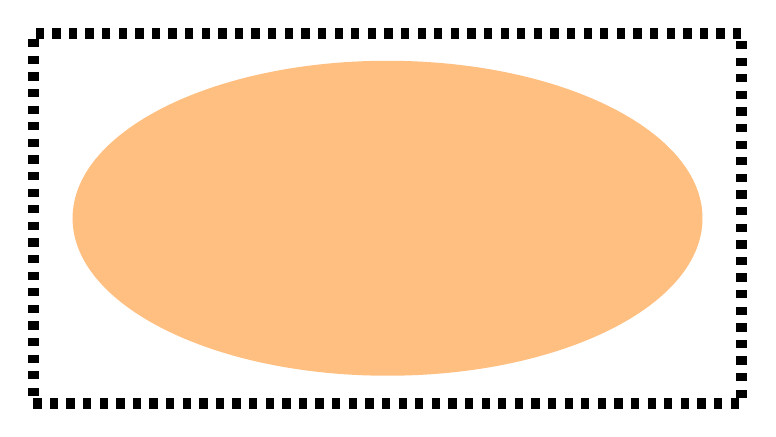
\begin{tikzpicture}
\draw [fill=orange!50,draw=none] (0,0) ellipse (4cm and 2cm);
\node[line width=4pt,dashed,rectangle,draw,minimum width=9cm,minimum height=4.7cm] at (0,0) {};
\end{tikzpicture}\par
1)~\textbf{over}-approximation
\par\columnbreak\par
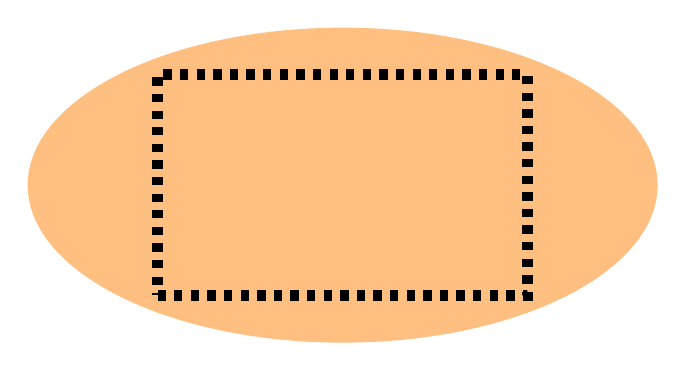
\begin{tikzpicture}[line width=2pt]
\draw [fill=orange!50,draw=none] (0,0) ellipse (4cm and 2cm);
\node[line width=4pt,dashed,rectangle,draw,minimum width=4.7cm,minimum height=2.8cm] at (0,0) {};
\end{tikzpicture}\par
2)~\textbf{under}-approximation
\end{multicols}

\plush{}

\pptSection[Functions]{Abstraction and Concretization}

\begin{pptWide}{3}
\emph{Concrete domain} \(C\) \\ \((\mathbb{Z}, <)\)\par
\begin{tikzpicture}[line width=1pt,->]
\node (a) {\(12\)};
\node [below=1cm of a] (b) {\(7\)};
\node [below=1cm of b] (c) {\(4\)};
\node [below=1cm of c] (d) {\(0\)};
\node [below=1cm of d] (e) {\(-9\)};
\draw (b) -- (a);
\draw (c) -- (b);
\draw (d) -- (c);
\draw (e) -- (d);
\end{tikzpicture}\par
\par\columnbreak\par
\emph{Abstract domain} \(A\) \\ \((\{s \vert \{ n \vert n \in \mathbb{N} \} \}, \in)\)\par
\begin{tikzpicture}[line width=1pt,->]
\node (top) {\(\mathbb{N}\)};
\node [below left=2cm of top] (2x) {\(2x\)};
\node [below right=2cm of top] (3x) {\(3x\)};
\node [below=2cm of 2x] (pow) {\(2^x\)};
\node [below=2cm of 3x] (6x) {\(6x\)};
\node [below=7cm of top] (bot) {\(\varnothing\)};
\draw (2x) -- (top);
\draw (3x) -- (top);
\draw (pow) -- (2x);
\draw (6x) -- (3x);
\draw (6x) -- (2x);
\draw (bot) -- (pow);
\draw (bot) -- (6x);
\end{tikzpicture}\par
\par\columnbreak\par
Abstraction function:\\
\(\alpha(c) \to a\)

Concretization function:\\
\(\gamma(a) \to c\)

Domains must be related through \emph{Galois connection}:
\(\forall c \in C, \forall a \in A\)\\
\(\alpha(c) \sqsubseteq a \Longleftrightarrow c \sqsubseteq \gamma(a) \)

\textcolor{red}{Are they?}
\end{pptWide}

\plush{}

\pptSection[Transformers]{Abstract Semantics (Transformers)}

\begin{pptWide}{3}
\emph{Abstract domain}:\par
\begin{tikzpicture}[line width=1pt,->]
\node (top) {\(\mathbb{N}\)};
\node [below left=2cm of top] (2x) {\(2x\)};
\node [below right=2cm of top] (3x) {\(3x\)};
\node [below=2cm of 2x] (pow) {\(2^x\)};
\node [below=2cm of 3x] (6x) {\(6x\)};
\node [below=7cm of top] (bot) {\(\varnothing\)};
\draw (2x) -- (top);
\draw (3x) -- (top);
\draw (pow) -- (2x);
\draw (6x) -- (3x);
\draw (6x) -- (2x);
\draw (bot) -- (pow);
\draw (bot) -- (6x);
\end{tikzpicture}\par
\par\columnbreak\par
Transformers:

\(\mathbb{N} + \mathbb{N} = \dots\)

\(2x + 2x = \dots\)

\(2x + 3x = \dots\)

\(2x \times 3x = \dots\)

\(\varnothing + 2x = \dots\)

\par\columnbreak\par
Concrete counterparts:

\(1024 + 1 = \dots\)

\(46 + 4 = \dots\)

\(8 + 9 = \dots\)

\(6 \times 12 = \dots\)

\(-1 + 4 = \dots\)
\end{pptWide}

\plush{}

\pptSection[Widening]{Widening and Narrowing}

\begin{pptWide}{2}
\begin{tikzpicture}[line width=1pt,->]
\node (top) {\(\top\)};
\node [below left=6cm and 2cm of top] (e) {\(\mathcal{E}\)};
\node [below right=1cm of top] (nn) {\(\mathbb{N}\)};
\node [below right=1cm of nn] (n) {\(\mathbb{N}_+\)};
\node [below left=1cm and 4cm of n] (zero) {\(0\)};
\node [below left=1cm and 2cm of n] (1) {\(1\)};
\node [below left=1cm and 0cm of n] (2) {\(2\)};
\node [below left=1cm and -2cm of n] (3) {\(3\)};
\node [below left=1cm and -4cm of n] (4) {\(4+\)};
\node [below=8cm of top] (bot) {\(\bot\)};
\draw (e) -- (top);
\draw (nn) -- (top);
\draw (zero) -- (nn);
\draw (n) -- (nn);
\draw (1) -- (n);
\draw (2) -- (n);
\draw (3) -- (n);
\draw (4) -- (n);
\draw (bot) -- (e);
\draw (bot) -- (zero);
\draw (bot) -- (1);
\draw (bot) -- (2);
\draw (bot) -- (3);
\draw (bot) -- (4);
\end{tikzpicture}\par
\par\columnbreak\par
\(0 \bigtriangledown 1 = \dots\)

\(1 \bigtriangledown \mathbb{N}_+ = \dots\)

\(0 \bigtriangledown \mathbb{N}_+ = \dots\)

\(1 \bigtriangleup \mathbb{N}_+ = \dots\)

\(0 \bigtriangleup 1 = \dots\)

\(3 \bigtriangleup 4+ = \dots\)
\end{pptWide}

\plush{}

\pptSection[Fixed-Point]{Fixed-Point Computation}

\emph{Fixed-Point Computation} is a repeated symbolic execution of the program using abstract semantics
until approximation reaches an \emph{equilibrium}.

\begin{pptWide}{3}
{\ttfamily
int f(int x) \{ \\
\quad while x > 0 \{ \\
\quad \quad x = x - 1;\\
\quad \quad x = 2 / x;\\
\quad \}\\
\quad return x;\\
\}}
\par\columnbreak\par
\begin{tikzpicture}[graph]
\node (start) {$\circ$};
\node[terminal,below=1cm of start] (while) {x > 0}; \path (start) edge (while);
\node[terminal,below=1cm of while] (minus) {x = x - 1}; \path (while) edge (minus);
\node[terminal,below=1cm of minus] (div) {x = 2 / x}; \path (minus) edge (div);
\node[left=2cm of minus] (exit) {$\circ$};
\path (div.east) edge [bend right=90] (while.east);
\path (while.west) edge (exit);
\end{tikzpicture}
\par\columnbreak\par
\begin{tikzpicture}[line width=1pt,->]
\node (top) {\(\top\)};
\node [below left=6cm and 2cm of top] (e) {\(\mathcal{E}\)};
\node [below right=0.5cm and 1cm of top] (nn) {\(\mathbb{N}\)};
\node [below right=0.5cm and 1cm of nn] (n) {\(\mathbb{N}_+\)};
\node [below left=1cm and 4cm of n] (zero) {\(0\)};
\node [below left=1cm and 2cm of n] (1) {\(1\)};
\node [below left=1cm and 0cm of n] (2) {\(2\)};
\node [below left=1cm and -2cm of n] (3) {\(3\)};
\node [below left=1cm and -4cm of n] (4) {\(4+\)};
\node [below=7cm of top] (bot) {\(\bot\)};
\draw (e) -- (top);
\draw (nn) -- (top);
\draw (zero) -- (nn);
\draw (n) -- (nn);
\draw (1) -- (n);
\draw (2) -- (n);
\draw (3) -- (n);
\draw (4) -- (n);
\draw (bot) -- (e);
\draw (bot) -- (zero);
\draw (bot) -- (1);
\draw (bot) -- (2);
\draw (bot) -- (3);
\draw (bot) -- (4);
\end{tikzpicture}\par
\end{pptWide}

\plush{}

\plush{\pptChapter[Literature]{Further Reading/Watching}}

Lecture by Patrick Cousot, on \href{https://www.youtube.com/watch?v=IBlfJerAcRw}{YouTube}

Mozilla wiki page on \href{https://wiki.mozilla.org/Abstract_Interpretation}{Abstract Interpretation}.

\href{https://www.cs.utexas.edu/~isil/cs389L/AI-6up.pdf}{Slide deck} of I\c{s}il Dillig.

\href{https://bblanche.gitlabpages.inria.fr/absint.pdf}{Introduction to Abstract Interpretation} by Bruno Blanchet.

\end{document}
